\chapter{Anforderungen und Entwurf}
\label{sec:draft}

Auf Grund der Komplexität und des unvermeidbaren Rechenaufwands, welche ein Theorembeweiser mit sich
bringt, ist es aus aktueller Sicht ausgeschlossen diese Arbeit zu größeren Teilen im Browser zu
verwirklichen. Die einzige von allen größeren Browsern unterstützte Skriptsprache ist zur Zeit immer
noch \acr{js}, die vor allem auf Grund der dynamischen Typisierung und der fehlenden
Parallelisierbarkeit um einige Faktoren langsamer ausgeführt wird als nativer Code.

Ein besonderer Vorteil, den die Anwendung gegenüber bisherigen Lösungen bieten soll, ist die
Mobilität. Das bedeutet, dass es von jedem Rechner mit Internetzugang und einem modernen Webbrowser
aus möglich sein soll, die Anwendung zu nutzen und auf eventuell bereits zu einem früheren Zeitpunk
an einem anderen Ort erstellten Theorien zugreifen zu können. Damit wird klar, dass die Projekte und
Theorien nicht lokal auf den einzelnen Rechnern verwaltet werden können, sondern an einer zentralen
,von überall aus erreichbaren Stelle gespeichert sein müssen. Die Entscheidung zu einem Client-
Server-Modell ergibt sich bei einer Webanwendung ohnehin automatisch.

Weil es sich bei der Webanwendung um eine Entwicklungsumgebung handelt, die insbesondere durch
Echtzeitinformationen einen Mehrwert bieten soll, ist einer der wichtigsten Aspekte des Entwurfs die
effiziente Kommunikation zwischen Server und Browser. Da die Kommunikation bei einer Webanwendung
generell sehr zeitaufwändig ist - abhängig von der Internetanbindung kann es zu großen Verzögerungen
kommen - muss abgewogen werden, welche Arbeit im Browser und welche auf dem Server erledigt werden
soll. Als illustratives Beispiel kann das Syntax-Highlighting genannt werden: Isabelle verfügt über
eine innere und eine äußere Syntax, die sich im analytischen Aufwand stark unterscheiden. Während
die äußere Syntax relativ leicht zu verarbeiten ist und dabei bereits viele Informationen liefert,
ist die innere Syntax sehr komplex, flexibel und stark vom jeweiligen Kontext abhängig. Somit liegt
es nahe, das Syntax-Highlighting aufzuteilen: Um Übertragungskapazität zu sparen, kann das
Highlighting der äußeren Syntax bereits im Browser mittels \acr{js} stattfinden. Die feiner
granulierten Informationen aus der inneren Syntax können dann auf dem Server ermittelt werden und
mit kurzer Verzögerung in die Darstellung integriert werden.

\section{Server}

Der Webserver muss neben den normalen Aufgaben eines Webservers, wie der Bereitstellung der Inhalte,
der Authentifizierung der Benutzer sowie der Persitierung bzw. Bereitstellung der Nutzerspezifischen
Daten (In unserem Fall Sitzungen / Theorien), auch eine besondere Schnittstelle für die Arbeit mit
den Theorien bereitstellen. Vom Browser aus muss es möglich sein, 

\begin{itemize}
  \item die einzelnen Theorien in Echtzeit zu bearbeiten,
  \item Informationen über Beweiszustände bzw. Fehler zu erhalten,
  \item als auch Informationen über die Typen, bzw. Definitionen von Ausdrücken zu erhalten.
\end{itemize}

All diese Informationen müssen zuvor Serverseitig aufbereitet und bereitgestellt werden. Dabei ist
es aus Sicht der Perfomanz wichtig, unnötige Informationen zu eliminieren und die Daten zu
komprimieren.

\TODO{Weitere Anforderungen an den Server}

\subsection{Wahl des Webframeworks}

Für die Realisierung des Webservers wählen wir das \textit{Play
Framework}\footnote{http://www.playframework.org} in Version 2.1. Da wir die Isabelle/Scala
Schnittstelle nutzen, liegt es nahe ein Webframework in Scala zu nutzen um den Aufwand für die
Integration gering zu halten. Als Alternative existiert das \textit{Lift
Webframework}\footnote{http://www.liftweb.org} welches allerdings auf Grund des Rückzugs von David
Pollack aus der Entwicklung seit einiger Zeit nicht mehr geordnet weiter entwickelt wird und zudem
für unsere Zwecke überdimensioniert ist. Da die Webanwendung eher unkonventionelle Anforderungen an
den Server hat, nutzen die meisten Funktionen von \textit{Lift} nichts. Das \textit{Play}
Webframework ist hingegen vorallem auf hohe Performance und weniger auf die Lösung möglichst vieler
Anwendungsfälle ausgelegt, womit es für unsere Zwecke interessanter bleibt.

\subsection{Authentifizierung}

Die Authentifizierung soll in diesem Projekt bewusst einfach gehalten werden, da es sich hierbei um
eine Nebensächlichkeit handelt, welche ohne weitere Probleme aufgerüstet werden kann. Wir
beschränken uns daher auf die Möglichkeit sich mit einem Benutzernamen sowie einem dazugehörigen
Passwort einzuloggen, welche dann mit einer Konfigurationsdatei auf dem Server abgeglichen wird. Wir
können dann auf die Möglichkeit des Play Frameworks zur sicheren Verwaltung von Session-Bezogenen
Daten zurückgreifen um die Anmeldung aufrechtzuerhalten.

\subsection{Persistenz}

Als Besonderheit bei der Datenpersistenz sind die serverseitig zu verwaltenden Theorien zu nennen.
Da jeder Benutzer eine von allen anderen Benutzern unabhängige Menge von Projekten mit Theorien
besitzt, also eine hierarchische Struktur besteht, spricht nichts dagegen, die Daten Serverseitig im
Dateisystem zu verwalten. Somit ist auch eine eventuelle spätere Integration eines
Versionsverwaltungssystems möglich. Da über diese Daten hinaus nur wenige Informationen vom Server
verwaltet werden müssen, ist die Einrichtung und Anbindung einer Datenbank nicht von Nöten.

\subsection{Bereitstellung von Resourcen}

Das Play-Framework bietet ausgefeilte Möglichkeiten sowohl statische als aus dynamische Resourcen
bereit zu stellen. Ein Hauptaugenmerk liegt hierbei auf der Bereitstellung der nötigen \acr{js}-,
\acr{css}- sowie \acr{html}-Dateien.

Während der Entwicklung dieser Arbeit wurde ein Modul für das Play Framework entwickelt, um \textbf
{CoffeeScript-Dateien} automatisch zu \acr{js} zu übersetzen, Abhängigkeiten mit RequireJS
aufzulösen und eine Optimierte \acr{js}-Datei bereitzustellen. Da in der in Kürze erscheinenden
Version 2.1 des Play Framework ganau diese Funktionalität entwickelt wurde, liegt die Entscheidung
nahe, diese Funktionalität zu nutzen und das eigene Modul wegfallen zu lassen. (Siehe
\ref{sec:play})

Ebenfalls von Play unterstützt wird die Möglichkeit  \textbf{\acr{less}-Dateien} mit ihren
Abhängigkeiten zu einer \acr{css}-Datei zu übersetzen. Da diese genau wie bei der CoffeeScript-
Übersetzung zur Entwicklungszeit in lesbare und im Produktiveinsatz in optimmierte Dateien übersetzt
werden, ist dies eine optimale Wahl.

\textbf{Statische Resourcen} wie in unserem Fall z.B. Font-Dateien oder fremde \acr{js}-Bibliotheken
werden durch einen sogenannten Asset-Controler aus dem Play-Framework bereitgestellt. Dieser bietet
die Möglichkeit alle Dateien in einem Ordner statisch bereitzustellen. In unserem Fall sind das die
Dateien im Ordner \texttt{"/public"} welche unter der \acr{url} \texttt{"/assets"} bereitgestellt
werden.

\subsection{Isabelle/Scala Integration}

\TODO{Isabelle/Scala auf dem Server}


\clearpage

\section{Kommunikation}
\label{sec:comm}

Da viele Daten in hoher Frequenz übertragen werden müssen, (Nach jeder Veränderung des Dokuments
muss der Server informiert werden, der dann zu unbestimmten Zeitpunkten in mehreren Schritten die
Zustands- Informationen zurücksendet) ist eine normale Datenübertagung wie bei Webapplikationen
üblich über \acr{ajax} bzw. \acr{http}-Anfragen nicht gut geeignet: Bei normalem \acr{http} ist es
zum einen immer nötig auf Browser Seite eine Anfrage zu stellen um Informationen vom Server zu
erhalten, zum anderen hat jede Anfrage und jede Antwort zusätzlich einen Header, welcher mindestens
einige hundert Bytes groß ist.

Als Worst-Case-Beispiel kann das Entfernen von Kommandos aus dem Dokumenten-Modell betrachtet
werden: Um das Modell eines Dokuments auf Server und Client synchron zu halten müssen ab und zu
Nachrichten vom Server gesendet werden, welche signalisieren, dass ein Kommando aus dem Modell
entfernt wurde. Diese Nachricht enthält als Information die eindeutige ID des Kommandos. Bei der ID
handelt es sich um eine 64-Bit Zahl. Zusätzlich dazu muss signalisiert werden, um welche Aktion es
sich eigentlich handelt. Dafür reichen bei der überschaubaren Anzahl an möglichen Aktionen weitere 4
Byte mehr als aus. Das bedeutet, die eigentlichen Informationen die für diese Aktion relevant sind
belaufen sich auf höchstens 12 Byte. Würde diese Aktion über \acr{http} laufen müsste zunächst eine
Anfrage gestellt werden

\begin{lstlisting}
GET /user/project/file.thy/remove-command HTTP/1.1
Host: www.clide.net
\end{lstlisting}

Diese Anfrage allein ist bereits 70 Zeichen lang ohne dass überhaupt relevante Informationen
übertragen wurden. Die minimale Antwort sähe dann in etwa so aus:

\begin{lstlisting}
HTTP/1.1 200 OK
Server: Apache/1.3.29 (Unix) PHP/4.3.4
Content-Length: 12
Content-Language: de
Connection: close
Content-Type: text/html

178
\end{lstlisting}

Das sind zusammen über 250 Zeichen um zu signalisieren, dass Kommando 178 entfernt werden soll.
Damit wurde die Information um den Faktor 30 aufgeblasen. Zusätzlich kommt es zu Verzögerungen durch
die zusätzlichen Anfragen. 

\subsection{Google SPDY}

Google experimentiert zu zeit mit einem neuen Protokoll für schnellere Webanwendungen bei dem die
Header komprimiert werden und vor allem unbegrenzt viele parallele Anfragen gestellt werden können.
SPDY führt zu einem drastischen Geschwindigkeitsgewinn bei der Arbeit mit vielen kleinen
Nachrichten. Das Protokoll ist jedoch zur Zeit noch experimentell und wird lediglich von einem
experimentellen Build des \textit{Google Chrome} Browsers unterstützt. Eine Unterstützung in Play
fehlt vollständig. Eine Implementierung, welche auf SPDY aufbaut wäre damit nicht von einer größeren
Nutzerzahl verwendbar. Darüber hinaus ist der Erfolg des Protokolls ungewiss.

\subsection{WebSockets}
\label{sec:ws}

Die im \acr{html}5-Standard eingeführten WebSockets sind die ideale Lösung für das Problem. Bei
WebSockets wird eine vollduplex Verbindung über TCP aufgebaut, welche ohne den HTTP-Overhead
auskommt und lediglich ein Byte pro Nachricht benötigt um zu signalisieren, dass eine Nachricht
endet. Außerdem ist es durch die duplex Verbindung möglich sogenannte Server-Pushes wie in dem
vorangegangenen Beispiel ohne vorheriges Polling bzw. eine verzögerte Antwort auf eine Anfrage zu
realisieren.

Dadurch, dass WebSockets ein relativ neues Konzept bilden, werden durch deren Anwendung die meisten
älteren Browser von der Benutzung der Webapplikation ausgeschlossen. Ein Fallback auf HTTP wäre zwar
relativ leicht zu implementieren, aber in der Benutzung kaum akzeptabel, da sich die zusätzlichen
Verzögerungen bei teilweise weit über 1000 Nachrichten pro Minute so negativ auf die
Ausführungsgeschwindigkeit auswirken würden, dass ein produktives Arbeiten mit dem System nicht mehr
möglich wäre. Aktuell werden WebSockets von allen relevanten Browsern in der neusten Version
unterstützt. Browser die seit einem Jahr nicht mehr aktualisiert wurden können mit dem Aufruf
allerdings zu großen Teilen nichts Anfangen. (Siehe Abschnitt\,\ref{sec:comp}) Das Play Webframwork
unterstützt Serverseitige WebSocket-Verbindungen. Allerdings muss bei der Benutzung auf viel
Funktionalität verzichtet werden. Da WebSockets allerdings so unabdingbar sind werden diese
Einschränkungen akzeptiert.

\subsection{Protokoll}

Für das Protokoll wurde zunächst der Einfachheit halber \acr{json} gewählt mit der Möglichkeit im
Hinterkopf, es zu einem späteren Zeitpunkt leicht durch das komprimierte \acr{bson}-Protokoll zu
ersetzen. Um das möglich zu machen wird unter Verwendung von Dynamischer Typisierung in Scala (Siehe
Abschnitt\,\ref{sec:dyn}) vom Übertragungsprotokoll abstrahiert, (Siehe Abschnitt\,\ref{sec:jsc})
damit es ohne größeren Aufwand ausgetauscht werden kann.


\clearpage

\section{Client}

Zur Realisierung des Clients wird auf die etwas komforablere Scriptsprache CoffeeScript
zurückgegriffen. CoffeeScript-Code is gegenüber \acr{js}-Code deutlich kürzer, (Etwa 30\%) und hat
eine an Funktionale Sprachen wie Haskell erinnernde Syntax. Da mit den neuen Möglichkeiten in Play
2.1 CoffeeScript problemlos verwendet werden kann (Der Browser erhält kompiliertes \acr{js}) ,
entstehen hierdurch keine Nachteile.

Zur Strukturierung wird RequireJS sowie BackboneJS (und damit implizit auch UnderscoreJS) verwendet.
Durch die vielfältigen Möglichkeiten dieser Bibliotheken ist es möglich den Code klar zu
modularisieren.

\subsection{Browserkompatibilität}
\label{sec:comp}

Auf Grund der in \ref{sec:ws} beschriebenen Notwendigkeit, kann auf WebSockets nicht verzichtet
werden. Damit sind die meisten älteren Browser nicht mit der Anwendung kompatibel. 

\begin{table}[h]
\centering
\begin{tabular}{rlllll}
                  & \textbf{Chrome} & \textbf{Safari} & \textbf{IE} & \textbf{Firefox} 
                  & \textbf{Opera} \\\hline
  WebSockets      & 14.0            & 6.0             & 10.0        & 11.0             & 12.1  \\
  History API     & 5.0             & 5.0             & 10.0        & 4.0              & 11.5  \\
  WebWorkers      & 4.0             & 4.0             & 10.0        & 3.5              & 10.6  \\
  CSS Transitions & 4.0             & 3.1             & 10.0        & 4.0              & 10.5  \\

\end{tabular}
\label{tab:comp}
\caption{Kompatibilität der gängigsten Browser mit den Verwendeten Standards}
\captionsetup{font={footnotesize,bf,it}}
  \caption*{Datein von caniuse.com}
\end{table}

\TODO{Kompatibilitäts-Tabelle}

Aus Tabelle \ref{tab:comp} ist zu entnehmen, dass alle weiteren in der Anwendung benutzten Standards
eine geringere oder die gleiche Anforderung an die Aktualität des Browsers haben. Da WebSockets ein
sehr neues Konzept sind,  dienen sie als Orientierung: Alle Features, welche von jedem Browser, der
WebSockets unterstützt, auch unterstützt werden, dürfen verwendet werden. Alle anderen schließen wir
aus, da sonst die Zahl der potentiellen Nutzer weiter eingeschränkt würde. Die Anwendung ist damit
im Standardbrowser auf allen Systemen mit einem aktuellen Betriebssystem (Windows 8, Ubuntu 12.10,
OpenSUSE 12.2, OS X 10.8.2), sowie auf dem iPad, und aktuellen Windows RT Tablets benutzbar. Bei der
Entwicklung wurde jedoch besonderes Augenmerk auf WebKit-basierte Browser, insbesondere Google
Chrome gelegt und einige der anderen genannten Systeme sind ungetestet und damit ohne Gewähr.

\subsection{Benutzeroberfläche}

Bei der Gestaltung des \acr{ui} wurde besonderes Augenmerk auf die User Experience gelegt
um die Produktivität und die Zufriedenheit der Nutzer zu optimieren. \cite{emotionaldesign}
Inspiriert wurde das Design durch die von Microsoft in Windows Phone 7 bzw. Window 8 eingeführte
Design Sprache \textit{Metro UI} (bzw. seit 2012 \textit{Microsoft Design Language}). \cite{metroui}
Dabei wird auf unnötige Grafiken verzichtet und die Typographie in den Vordergrund gestellt. Durch
die Reduktion auf das Wesentliche entsteht eine neue Ästhetik welche eine willkommene Auffrischung
der Icon- und Fensterbasierten Oberflächen wie sie seit jeher bestehen, bietet.

\begin{figure}[ht]
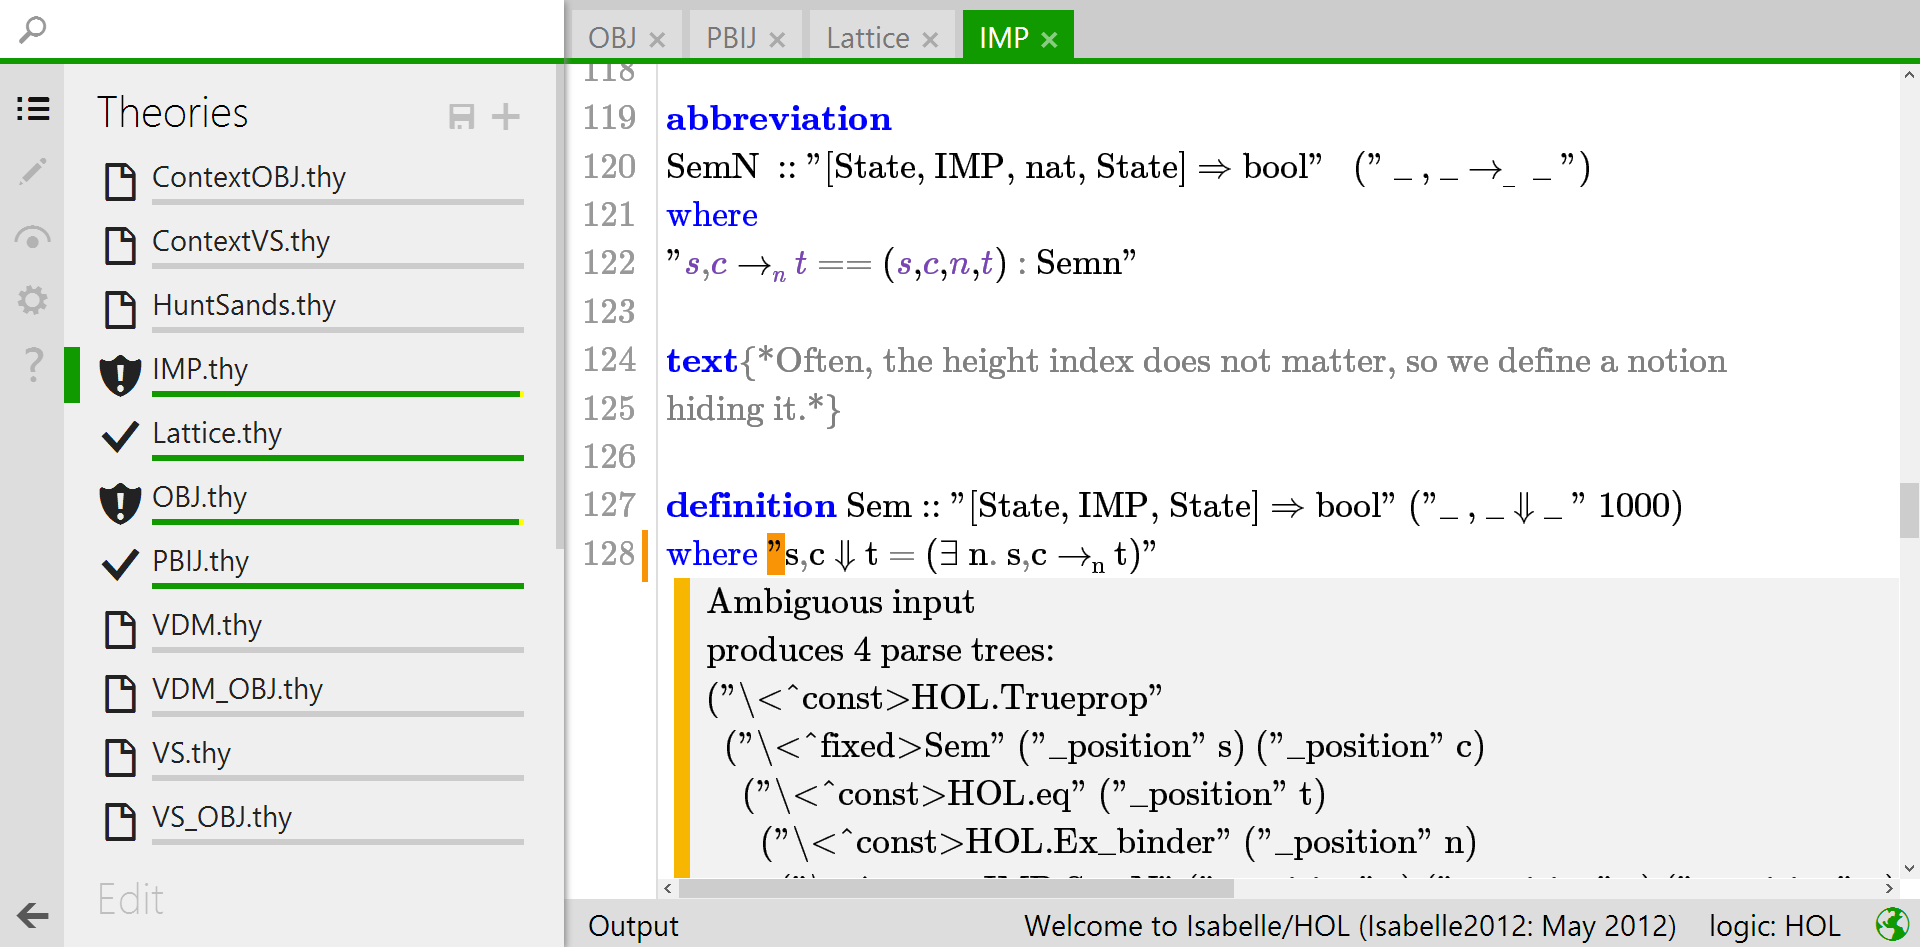
\includegraphics[width=\linewidth]{images/screen-main}
  \caption{Die clide-Oberfläche}
  \label{fig:screen-main}
\end{figure}

Besondere Herausforderungen sind das sinnvolle Unterbringen der Beweiszustände und
Fehlerinformationen in der Darstellung sowie die Darstellung des Fortschritts, der einzelnen
Theorien, welche nicht zwingend vom Nutzer geöffnet werden müssen sondern auch implizit als
Abhängigkeiten anderer Beweisdokumente verarbeitet werden können.

\subsubsection{Login}

Der Anmeldebildschirm (Login) ist entsprechend einfach gehalten. Dem Nutzer wird lediglich ein
Formular zur Eingabe von Benutzernamen und Passwort präsentiert. (Siehe Abbildung 
\ref{fig:screen-login})

Die Kommunikation erfolgt an dieser Stelle noch über normales \acr{http} und bei Fehlerhaften
Eingaben wird auf einer neu geladenen Seite eine Fehlermeldung über dem Formular angezeigt. Das
stört an dieser Stelle nicht und eine Nutzung von WebSockets würde die Sache hier nur
verkomplizieren, da so nicht die bereits ausgereiften Verfahren zur Anmeldung über \acr{http}
genutzt werden könnten.

\begin{figure}[ht]
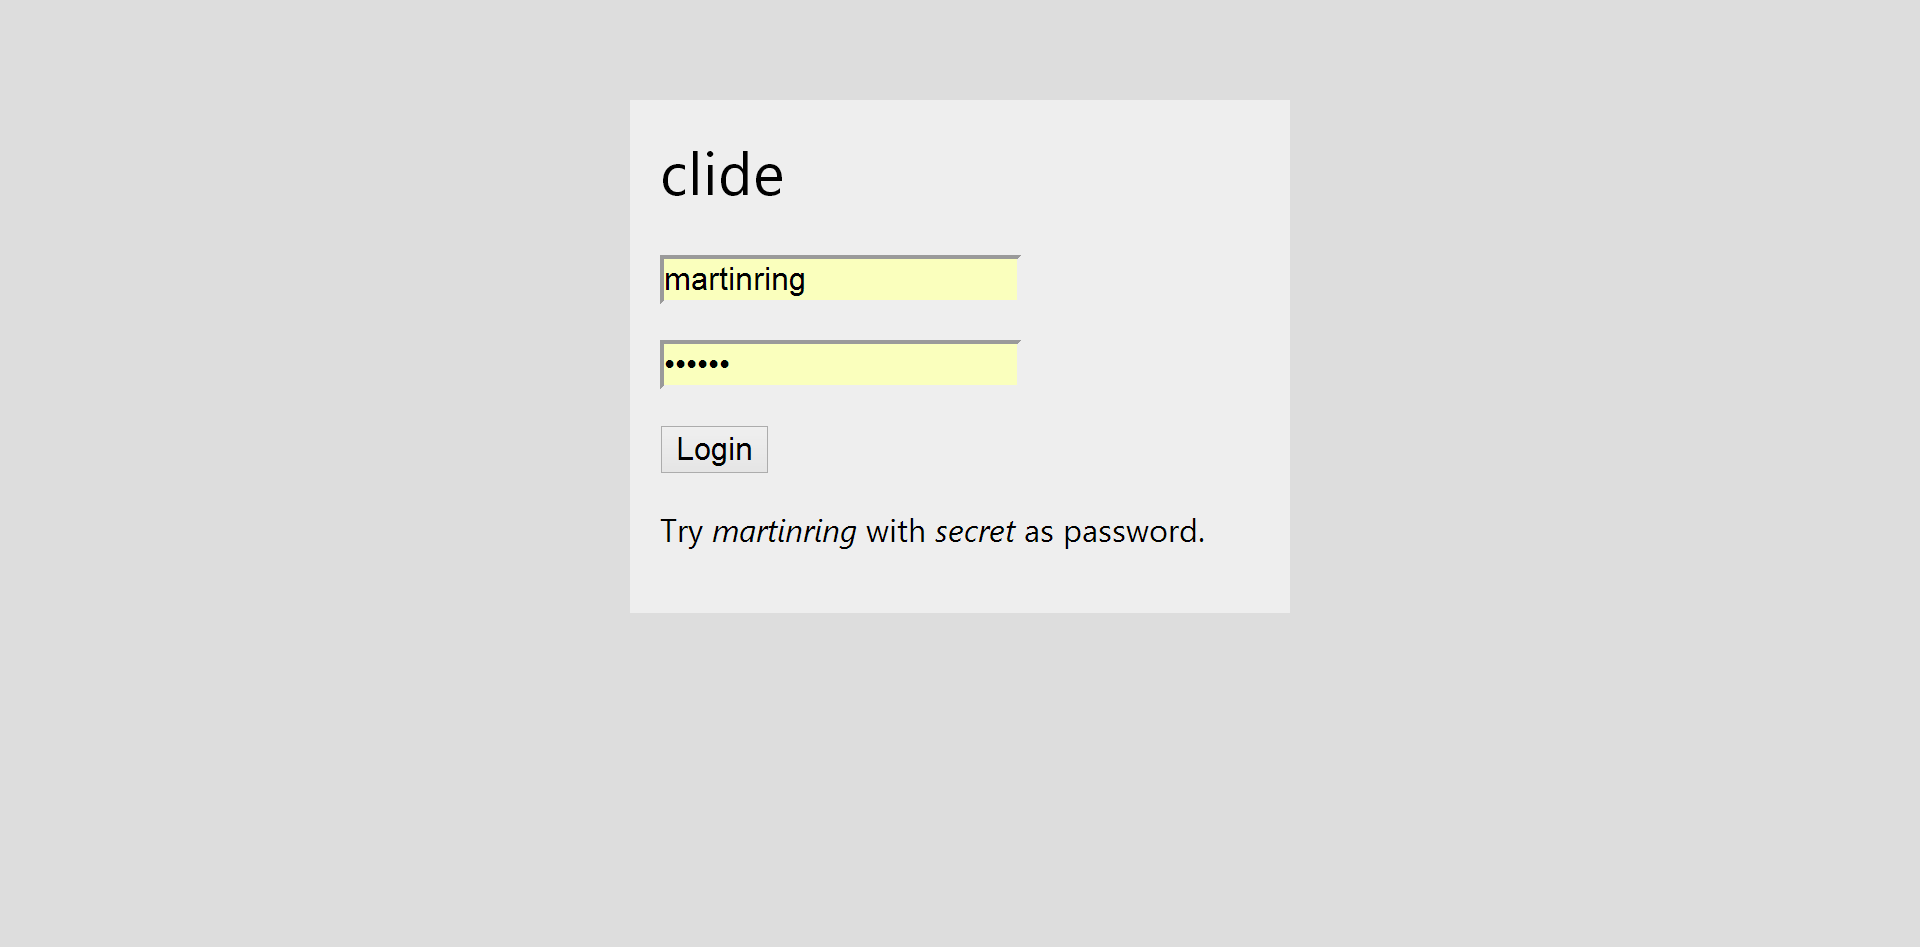
\includegraphics[width=\linewidth]{images/screen-login}
  \caption{Das Anmeldeformular}
  \label{fig:screen-login}
\end{figure}

\subsubsection{Projektübersicht}

\begin{figure}[ht]
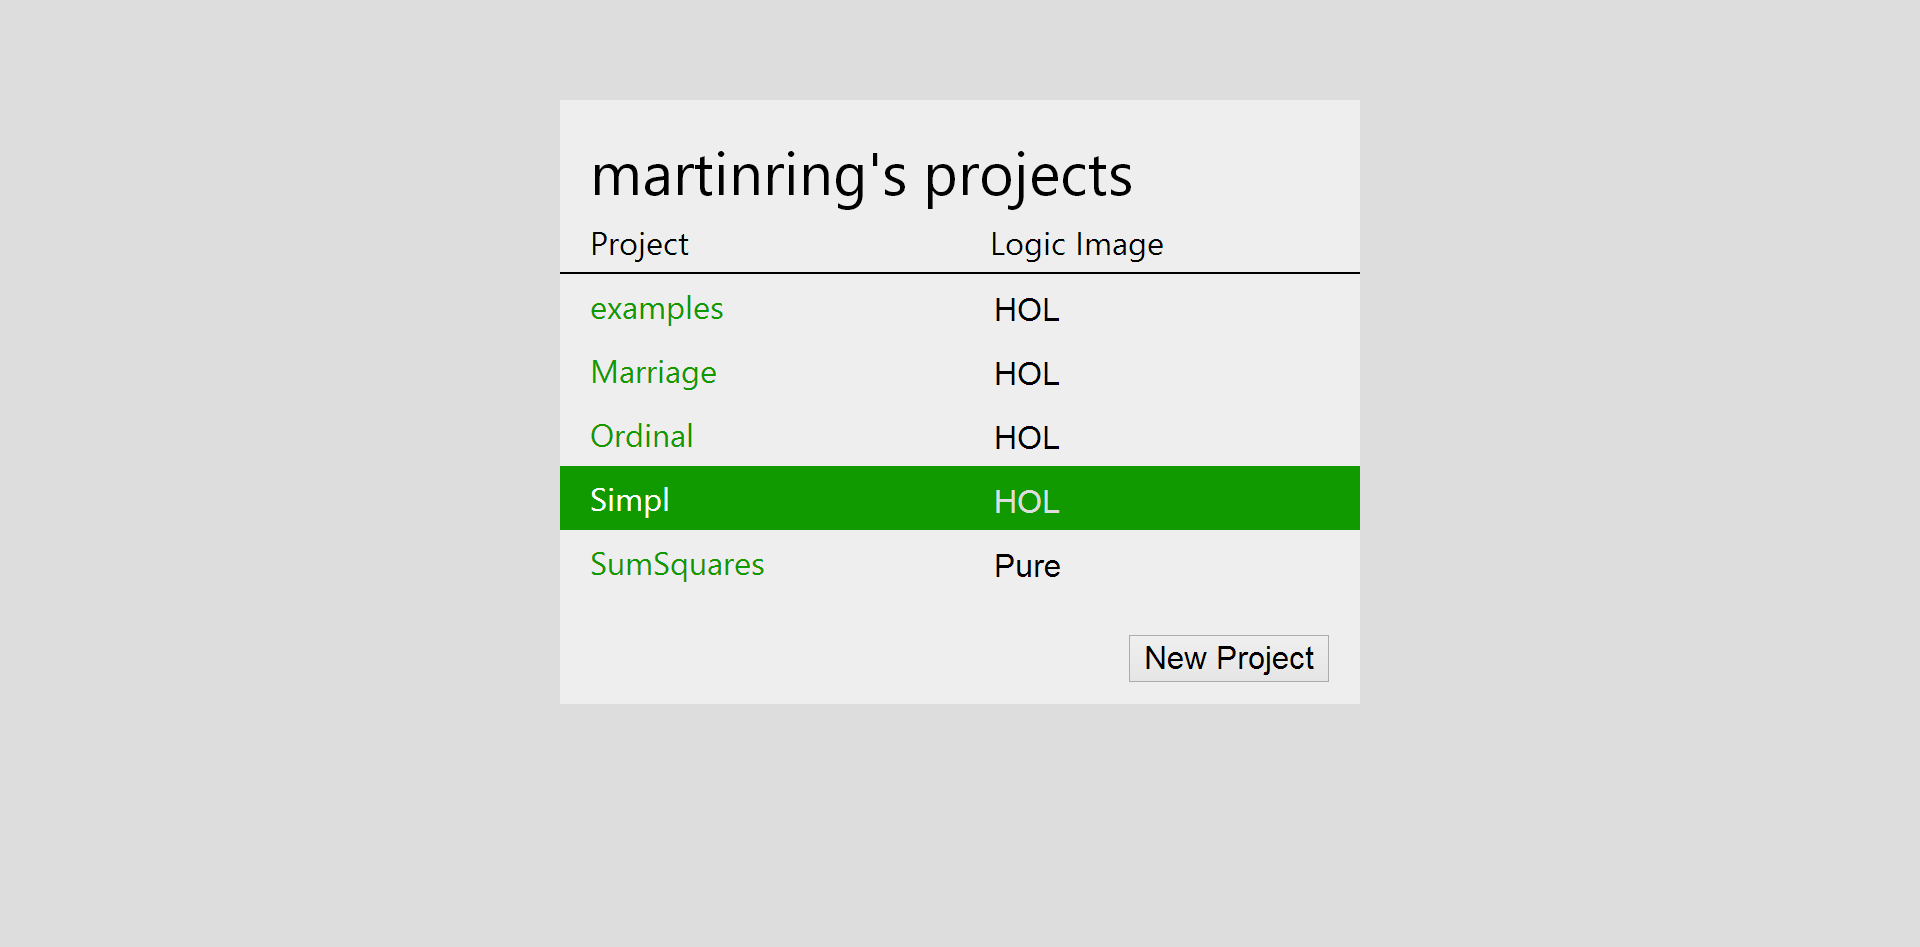
\includegraphics[width=\linewidth]{images/screen-projects}
  \caption{Die Projektübersicht}
  \label{fig:screen-projects}
\end{figure}

\subsubsection{Die Sidebar}

\begin{figure}[ht]
\centering
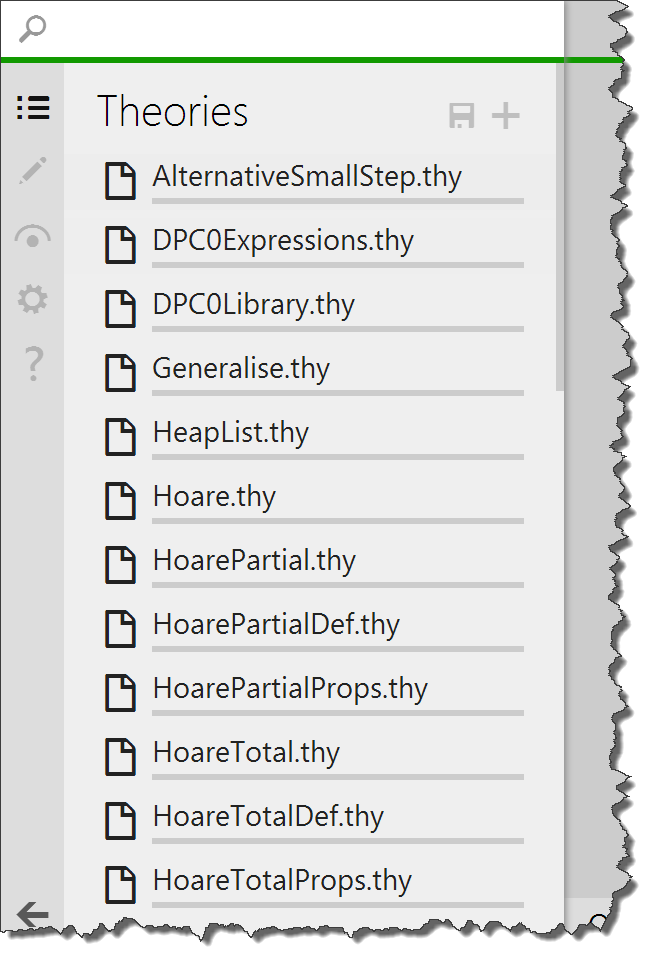
\includegraphics[width=0.4\linewidth]{images/screen-sidebar}
  \caption{Die Sidebar}
  \label{fig:screen-sidebar}
\end{figure}

\subsubsection{Die Editor-Komponente}

Die wichtigste Benutzerkomponente einer Entwicklungsumgebung ist der Text-Editor. Ein Editor für
Isabelle-Code hat hierbei besondere Anforderungen: Während in der Praxis bislang nur rudimentäre
Unterstützung für die Darstellung von Isabelle-Sonderzeichen und insbesondere von Sub- und
Superskript existierte, hat Isabelle/jEdit bereits eine stärkere Integration dieser eigentlich recht
essentiellen Visualisierungen eingeführt. \cite{iscala} Da bei der \acr{html}-Darstellung kaum
Grenzen gesetzt sind und sich \acr{css}-Formatierung sehr leicht dazu benutzen lässt bestimmte Text-
Inhalte besonders darzustellen, ist es klar, dass unsere Entwicklungsumgebung an dieser Stelle
besonders glänzen soll.

In einem ersten Prototypen war es möglich eine \acr{js}-Komponente zu entwickeln, welche es zuließ,
Isabelle-Code zu bearbeiten, sodass Sub- und Superskript sowie die Sonderzeichen korrekt dargestellt
wurden und bearbeitet werden konnten. Die besondere Anforderung bei ist hierbei nicht die
Darstellung sondern vor allem der Umgang mit den variablen Breiten. Selbst wenn ein Monospace-Font
verwendet würde, besteht das Problem, dass z.b. bei Sub- und Superskript nach Typographischen
Standards nur 66\% der Textgröße verwendet wird und somit auch die Zeichenbreite geringer wird. Da
aber eben die Visualisierung eine besondere Stärke der Anwendung sein soll, wollen wir zusätzlich
auch nicht darauf verzichten Ähnliche Fonts zu verwenden, wie in der Ausgabe der LaTeX-Dateien, also
auch Mathematische Sonderzeichen nicht in ein Raster quetschen. 

Eine weitere besondere Anforderung, welche bislang relativ einmalig zu sein scheint, ist die
Tatsache, dass das Syntax-Highlighting zu Teilen auf dem Server stattfinden soll und somit eine
Möglichkeit bestehen muss diese zusätzlichen Informationen in die Darstellung zu integrieren.

Zusammenfassend können folgende besondere Anforderungen an die Editor-Komponente formuliert werden:
Der Editor muss in der Lage sein

\begin{itemize}
  \item Syntaxhighlighting zu betreiben,
  \item Externes Syntaxhighlighting verzögert zu integrieren,
  \item Schriftarten mit variabler Zeichenbreite anzuzeigen,
  \item Tooltips für Typinformationen o.ä. anzuzeigen und
  \item Isabelle-Sonderzeichen zu substituieren.
\end{itemize}

Da der Hauptsächliche Aufwand bei einer Editor-Komponente nicht darin liegt Text zu bearbeiten und
darzustellen sondern vor allem in der Infrastruktur drumherum (Copy/Paste, Suche, Selektieren,
Drag'n'Drop, usw.) ist es verlockend, eine fertige Komponente zu verwenden. Hier existieren mehrere
ausgereifte Alternativen. Bei genauerer Betrachtung gibt es jedoch keine, welche optimal für unsere
Zwecke geeignet ist. 

\begin{description} 

\item {Der \textbf{MDK-Editor}\footnote{http://www.mdk-photo.com/Editor/}} bietet viele Features, wird
aber seit 2008 nicht mehr weiter entwickelt und scheidet damit sofort aus.

\item {Der \textbf{\acr{ace}}\footnote{http://ace.ajax.org/}} (Ehemals Mozilla SkyWriter) wird
momentan sehr stark weiter entwickelt. \acr{ace} bietet bereits ein ausgeklügeltes Framework für das
Syntaxhighlighting, welches sich in einem Prototyp relativ leicht an das Serverseitige
Syntaxhighlighting anbinden ließ. \acr{ace} bietet alle Funktionen, welche man von einem Modernen
Text-Editor erwartet, hat jedoch einen entscheidenden Nachteil: Zur Darstellung wird aus
Performance-Gründen intern ein festes Raster verwendet. Dabei wird davon ausgegangen, dass ein
Monospace Font verwendet wird. Von diesem wird einmalig eine Zeichenbreite ermittelt und diese feste
Metrik wird dann für alle internen Operationen verwendet. Da diese Designentscheidung so
tiefgreifend ist, scheint es nicht realistisch in akzeptabler Zeit, die Komponente so zu
modifizieren, dass variable Breiten unterstützt werden können. Außerdem ist es nicht möglich
Textstellen durch Sonderzeichen zu Substituieren. Somit scheidet auch \acr{ace} für die Verwendung
in der Anwendung aus.

\item {\textbf{CodeMirror}\footnote{http://codemirror.net/}} ist ebenfalls eine weit entwickelte
Editor-Komponente, welche nicht ganz so umfangreich, wie acr{ace} ist, jedoch um einiges flexibler
erscheint. In einem Prototyp war es möglich einige eigene Modifikationen für die Darstellung (Sub-
Superskript, Tooltips, Hyperlinks) zu integrieren. CodeMirror verwendet kein festes Raster, darunter
leidet die Performanz. Da wir jedoch darauf angwiesen sind, müssen wie diese Einbußen in der
Geschwindigkeit akzeptieren. Seit Version 3.0 welche am 10.12.2012 erschien, ist es möglich
Textteile zu durch HTML- Widgets zu substituieren. Dadurch ist es möglich Isabelle Sonderzeichen
welche durch ASCII Sequenzen wie beispielsweise \texttt{\textbackslash\textless
rightarrow\textgreater} für das Zeichen $\rightarrow$ repräsentiert werden direkt im Editor zu
ersetzen, sodass der bearbeitete Text valider Isabelle-Code bleibt, die Darstellung hingegen der
eines LaTeX-Dokuments entspricht.

\end{description}

Weitere Editoren existieren zwar, scheiden aber alle aus, da die meisten nicht einmal die Hälfte der
oben formulierten Anforderungen erfüllen. Es wird klar, dass CodeMirror der am besten geeignete
Editor ist. Trotzdem müssen einige eigene Anpassungen in den Kern des Editors integriert werden.
Diese sind unter anderem die Unterstützung von

\begin{itemize}
  \item Sub- und Superskript (sowie angepassten Cursorpositionen und -höhen),
  \item Tooltips für einzelne Textabschnitte sowie
  \item die Darstellung von Hyperlinks im Text.
\end{itemize}

\subsubsection{Beweiszustände}

\subsection{Client-Modell}

Der Client muss zu jeder Zeit über ein konsistentes Abbild der relevanten Informationen verfügen.
Das stellt sich als schwierige Herausforderung heraus. Insbesondere müssen der Inhalt des
Texteditors mit dem Server synchron gehalten werden. Abbildung \ref{fig:diagram-workflow} zeigt ein
Vereinfachtes Abbild des Datenflusses in der Anwendung. Die besondere Schwierigkeit liegt darin,
dass natürlich nicht jeder Tastendruck übertragen werden kann. Das würde auch wenig Sinn machen, da
es nicht realistisch ist, jede einzelne Veränderung zu überprüfen. Den Nutzer würden Fehlermeldungen
zu Zwischenzuständen stören und der Server wäre absolut überlastet. Also wird nach jedem Tastendruck
ein \textit{Timeout} von 700 Millisekunden gestartet. Wenn es abläuft, ohne dass eine Taste gedrückt
wird, werden die Veränderungen im Dokument an den Server übertragen. In dem häufigen Fall eines
weiteren Tastendrucks innerhalb der Zeispanne, wird das Timeout neu gestartet (\textit{Reset}) so
lange, bis der Nutzer über den Zeitraum von 700ms keine Veränderung mehr vornimmt.

Die Zeitspanne von 700 Millisekunden hat sich in eigenen Experimenten als guter Wert herausgestellt
und ähnliche Werte werden auch von anderen Entwicklungsumgebungen und Editoren (\acr{ace}, eclipse,
Visual Studio, ...), Standardmäßig verwendet um den Präsentationskompiler zu entlasten.

\TODO{Client-Modell}